\section{Introduction}

In order to meet exponentially growing consumer demand for wireless data, radio spectrum regulators considering opportunistic spectrum access policies. Historic spectrum regulation focussed on exclusive frequency assignments (licensing), with spatial and frequency separation to mitigate interference between users. However, this approach leads to considerable underutilisation in both space and time. Thus, faced with a need to provide 1000 times the bandwidth in 10 years, regulators are considering agile access technologies on a licence exempt basis.

Before opportunistic access is a reality, speedy, robust, and accurate estimation of frequency spectra must be made. This is a challenging statistical and engineering problem, limited by characteristics of wireless channels such as multipath fading, and shadowing. The proposed bands have a large bandwidth, containing sub-channels which are not contiguous but statistically correlated, and radio-wave fading environment which can mask high-powered transmissions. Traditional methods are un-viable in these conditions; either requiring expensive hardware to meet the data rate required to perform the sampling, or a large number of RF components to turn a single wideband channel into many narrowband ones.

This project addresses the issue of estimating available frequencies for opportunistic transmission, from a set of underdetermined measurements. The compete set of measurements may be available to a particular sensor. Or, the measurements may be distributed over a network of sensors, improving estimation accuracy, and 

The growing number of wireless devices is placing increasing demand on radio spectrum. Consumers are demanding faster speeds and better quality connections in more places. However, there is a limited amount of frequencies to transmit on. Consequently, demand for frequencies which provide sufficient bandwidth, good range and in-building penetration is high.

Not all frequencies are used at all times and in all places. Judicious spectrum management could alleviate the issue of too few frequencies being available to devices by developing approaches to interleaving opportunistic transmissions within established bands. 

There are benefits to spectrum sharing beyond simply satisfying consumer demand. Innovative wireless applications such as wireless rural broadband, remote monitoring, and machine-to-machine applications will be made viable without the need to purchase exclusive access to a specific frequency. 

The historic allocation process has placed unused spectrum between adjacent radio channels, in an attempt to avoid interference between consecutive users. However, technical changes in transmission standards are making some bands available as modern coding and modulation techniques are more spectrally efficient. In particular, in the UK, the switchover from analogue to digital terrestrial broadcast has freed many previously used bands.

Recent regulatory focus has been on frequencies in the TV broadcast bands 470-790MHz. In the UK, TV channels are broadcast using up to six multiplexes, each requiring an 8MHz channel. A total of 32 of these channels are allocated for TV broadcast, whilst only 6 of these channels are required to receive the 6 multiplexes at any given location. This is because TV broadcast is high powered and needs spatial separation between coverage areas to avoid interference. As such, the majority of TV frequencies reserved for TV broadcast are unused in any given place. These white spaces are spectrum which has been left over to prevent interference between primary users (such as TV broadcast). These frequencies can be used on an opportunistic basis by relatively low-powered devices. Whilst current focus is on the TVWS bands, the work presented in this thesis can be used in other, as yet unrealised frequencies.

Currently access to spectrum is managed in two ways: licensed and license exempt access. Licensing authorises a particular user/users to exclusive use of a specific frequency band. License exempt access allows any user to access a band, provided they meet technical requirements intended to limit interference in on other users. This is a particularly pressing issue for the co-existence of licensed users and licence exempt users in the same band.

Devices seeking to access white spaces need a robust mechanism for learning which frequencies can be used at a particular time and location. The approach currently being taken by OFCOM and the FCC is to maintain a set of databases, which map the location of white spaces based on knowledge of existing spectrum users. An alternative approach is for devices to monitor the use of spectrum individually.

One approach to white-space access is to maintain a database of currently available frequencies. The database would contain up to date information about incumbents, including television transmitters and wireless microphones. It would also need to maintain information about currently operative secondary users. Devices would register with the database, based on their geo-location and the service would determine availability for the device, either based on in situ measurements, or from a propagation model.

Location based measurements are a costly approach, as they need to be redone every time primary user transmission characteristics change, and they cannot be done economically in difficult to reach places. Propagation models can achieve good accuracy, but at the cost of being complex and computationally intensive. Simplistic models do not agree with ground truth measurements. 

Devices must also supply geographic information to a database service. How this is done has yet to be codified, but current methodologies all have drawbacks. GPS positioning works well outdoors, but is inaccurate indoors. Cellular location can yield errors of up to a mile. Using the base-station location as a proxy for the device location results in an unacceptably high loss of whitespaces, as decisions would have to be needlessly conservative.

An alternative to maintaining a database of available frequencies, is for secondary users to independently sense spectrum. This method is subject to a number of technical limitations. The proposed bands have an ultra-wide bandwidth. Traditional sensing approaches to this have been either to divide the band into a number of contiguous narrow bands, or to simply use a high rate processing device to capture the necessary samples. Both methods are prohibitively expensive, and require dedicated and energy hungry hardware. Further, traditional statistical spectral detection and estimation techniques make assumptions about the primary users signal. Such assumptions include cyclo-stationarity, the presence of specific waveform patters, the use of known pilot sequences, and sufficiently high powered transmissions that energy detection is viable. In practice, some (or all) of these assumptions are violated; either because assumed patterns are not present in the  transmission, or because the radio environment has a deep fade between the primary and secondary user masking high powered transmissions.

The biggest issues for single node sensing are multipath fading, shadowing, and PU receiver uncertainty. Cooperation between a network of nodes can improve sensing performance through spatial diversity. In cooperative sensing information from geographically diverse nodes is aggregated in the decision making process. Combining observations can overcome the deficiencies of observations unique to individual cognitive radios. Spatial diversity makes it unlikely that all radios will experience the same fading and receiver uncertainty. Approaches to cooperative sensing based on Nyquist sensing typically involve energy detection at each node, along with a gain combining procedure (which is either performed at a fusion node, or via a decentralised algorithm). Cooperative sensing can use such simple methods at each node as receiver sensitivity can be mitigated by using multiple statistically independent observations. This reduces the complexity and cost of the individual cognitive radios.

Cooperative sensing has drawbacks however. Spatial diversity does not necessarily mean statistically independent observations. A subset of nodes all blocked by the same object will make measurements which are correlated and corrupted by the same shadowing for example. Cooperative sensing also involves an overhead with the being part of a network. This is any extra time, energy and processing when compared to sensing individually. 

An alternative sensing strategy is compressive sampling (CS). This is a new paradigm in signal processing which has emerged over the last decade, and has had significant success in imaging problems. In particular compressive sampling strategies have reduced the time needed for an MRI scan from 2 minutes to 30 seconds. Patients previously had to hold their breath for the entire duration. The central innovation in compressive sensing is that randomness is an effective strategy for sensing sparse signals. In practice much of the TVWS spectrum is unoccupied, and CS can leverage this sparsity to reduced the sampling rate of the CRS.

Group Testing is a model sparse inference problem, first introduced by Dorfmann in the context of testing for rare disease. Given a population of items, some small fraction of which has an interesting property (labelled defective), Group Testing proposes algorithms to find those items efficiently. What allows these items to be discovered, in fewer tests than the total number of items, is testing pools of items. That is, items aren't tested individually, but several together. In testing for rare diseases the blood samples are mixed and the mixture is tested. This allows fast elimination of non-defective items. Popular pooling designs are randomised - items are included in a test with independent probabilities. We consider probabilistic algorithms with non uniform probabilities of each item's defectivity. These non-uniform priors could come from a TVWS database of possibly occupied spectrum, or from summarising risk and family history in disease testing.

In this thesis, we argue that in order to perform spectrum sensing n the TVWS band, at reasonable sampling rates we must exploit the new sensing paridigm of compressive sensing. We show how we can quantify the reduction in absolute number of samples needed to accuractely reconstruct a signal using this methodology. We diwcuss how the sample rate at a single node may still be too high even with the reduced rate, and we provide two approaches to reducing it even further. We also  discuss how with use the TVWS band may no longer be sparse, in the frequency basis. To recify this, we propose a distributed model of the spectral gradient, which allows us to accurately reconstruct the frequency bamd. We do this via an improved version of distributed ADMM. To reduce the smapling rate at a single device, we propose to aviod reconstruction altogether. We show it is possible to determine whether a frequency range is occupied with as little as 5% of the samples required by Nyquist sampling.  

The structure of this thesis is as follows. Chapter 2 covers the relevant material on Nyquist sensing theory and Nyquist approaches to the spectrum sensing problem. Nyqusit sensing is introuduced, and how to reconstruct the signal from its samples is covered. Then, what the spectrum sensing problem is is defined, along with narrowband approaches such as energy detection, feature detection, and matched filtering - in order of increasing complexity. Distributed and cooperative approaches to the problem are then dicussed, in particular the AND and OR rules of equal gain combining. We discuss that distrbuted approaches have better statistical performance due to spatial diversity, but that each sensor still needs to use the same number of samples as the single sensor problem. It is argued that the data rates demanded by TVWS sensing makes this Nyquist approach unfeasible, and that some mechanism of reducing the absolute number samples is required for spectrum sensing in the TVWS band to be a reality. 

Chapter 3 covers the theory of compressive sensing and some previous applications to the Wideband Spectrum sensing. In particular, the conditions under which a sparse high-dimensional vector can be recovered from undersampled representations are introduced - the Restriced Isometry Property (RIP) and stable embeddings along with which sensing operators satisfy these conditions. Then three families of reconstruction algorithm are discussed: greedy, convex and Bayesian. The relative merits and demerits of these alogorithms are compared in terms of speed, accuracy, complexity, and undersampling performance are discussed, concluding that more accurate algorithms which can reconstruct from fewer samples are slower and more complex. Two compressive approches to Wideband Spectrum sensing are then discussed in depth: the Random Demodulator and the Modulated Wideband Coverter, before moving on to discuss distributed compressive sensing.  

Chapter 4 covers the theory of ADMM. It starts with the a potted history of the algorithm - from solving the heat equation to optimisation in Hilbert spaces - and some applictaions, including imaging and predictive control problems. Then the theory of the Proximity operator is covered, and its connection to ADMM, along with examples pertinent to high-dimensional statistical signal processing. The introduction of the Prox operator is motivated by how it allows simple calculation of the sub-problems in ADMM. Thus, difficult non-smooth optimisation can be quickly performed in simpler stages.

Chapter 5 is new material and covers the application of and optimisation on graphs.

Chapter 6 introduces a model of 

Chapter 7 covers compressive inference

Chapter 8 covers the application of our methods to real world data sets.

Finally, Chapter 9 covers group testing and our approach to .

Despite the ubiquity, capacity and apparent efficacy, modern communication systems are wasteful, inefficient and in need of reform. Most of the bits of data collected by our sensing systems are unessential, and only serve to necessitate data compression wasting computation time before transmission. For example, people regularly use a camera with a resolution of several megapixels only to upload a file of a few kilobytes to Facebook. Devices are unable to make dynamic decisions about how to transmit this data, leading to both spectral exhaustion on some frequencies whilst much of the available radio spectrum lies fallow. 

This project addresses these issues, by reviewing a novel acquisition and decompression framework for data: a way in which we need only sense the most informative bits of data. This framework is then applied to the problem of sensing spectral opportunities dynamically, to make better use of available spectrum. 

The key uniting both these applications is that data and spectra are \textit{sparse}: that is they have a representations which are 'smaller' than their respective dimension. For example, images and audio can be compressed into file formats much smaller than when initially recorded (compare the relative sizes of bitmap and JPEG images).

The sole focus of this research is to use the sparsity of the spectrum to uncover transmission opportunities, allowing better use of spectrum more generally. 

We are motivated by the need to send more data over wireless networks, whilst at the same time having a constrained frequency set over which to transmit this information. This issue could be alleviated by users dynamically allocating spectrum on a per-transmission basis: without the ability to gain knowledge of spectral conditions this can never become a reality however. 

The requirement for increasing bandwidth isn't just a pressing issue for today: in the next decade it is forecast that network operators will need to provide for three-orders of magnitude (1000 times) more capacity. Demand is continually outstripping supply - motivated by the ubiquity of smart-phones, and the consumers appetites for media. 

At the same time as this demand for ever more data, there is an increasing scarcity of radio spectrum over which to transmit. New frequencies are rarely cleared for commercial purposes, and when they are they go for high prices.  A decade ago the UK auction for 3G spectrum licenses raised an estimated 22.4 billion pounds for the UK treasury, indicating the seriousness of the market players requirements for new spectrum. The recent 4G spectrum auction raised 2.3 billion pounds with initial networks being rolled out by the end of 2013.

\begin{figure*}[h]
\centering
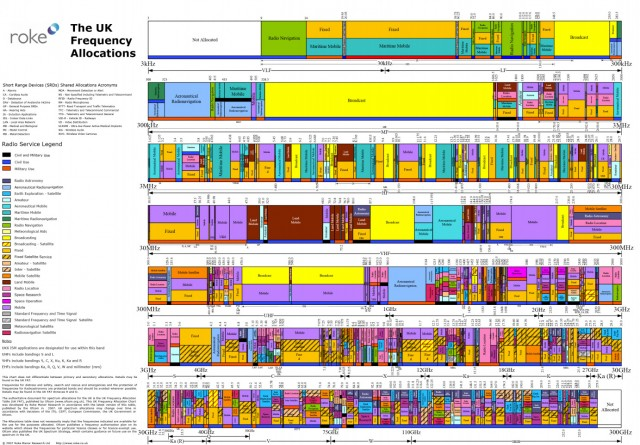
\includegraphics[height = 7 cm]{uk-spectrum-allocation-chart1-640x445.jpg}
\caption{A digram of current Spectral allocation \cite{Strategy2013}}
\label{spectrumalloc}
\end{figure*}

However, a closer inspection of the frequency allocation suggests this scarcity is artificial, it's more a product of regulatory oversight over time. As the constraints on spectrum requirement became more complex, so did the solutions to that problem - at the cost of leaving much of the spectrum idle for most of the time. 

For example: much of the spectrum is allocated to TV broadcast, radio broadcast and mobile. However, if we look closer, the allocations aren't even for specific companies - they're simply categories. Within these, OFCOM may have many licensees within each category.

Also interesting to note is how much frequency the Government allocates to itself (the red bar underneath the blocks indicates Government use). Compare this to the actual utilisation of spectrum: much of it is not used at all. Figure \ref{frequtil} shows a snapshot of frequency utilisation in three diverse locations in the UK over te radio specturm, note that many frequencies are not utilised (coloured blue) whilst others have significant activity (coloured yellow). Note that the plot for Southwark (central London) is barely different from Braddock - a rural area. 

\begin{figure*}[h]
\centering
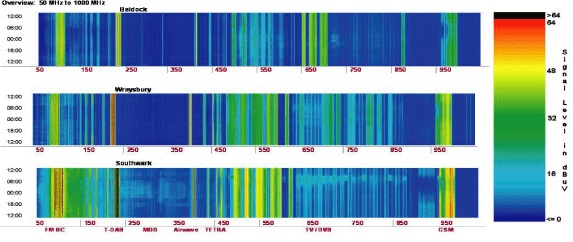
\includegraphics[height = 7 cm, width=0.5\textwidth]{cr2.jpg}
\caption{A snapshot of frequency utilisation in various areas: many frequencies are not used at all, whilst there is significant activity on others \cite{Burbidge2007}}
\label{frequtil}
\end{figure*}

How do we then go about solving this issue - how can we obtain the most significant bits of information from our sensing mechanism, whilst obviating the need to compress the data once we are done? How do we dynamically assign spectrum? The work of Candes, Tao \cite{Candes2006} and Donoho \cite{donoho2}, has shown that instead of measuring the information we require directly (and then compressing it), we can measure 'holographic' and non-linear random projections between our measurement space and the space where our data is sparse. This requires only the knowledge that the signal is compressible via some transform - both the acquisition protocol and the reconstruction algorithm are agnostic to the type of signal. What is surprising is that the sampling kernels are fixed independently of the signal, are non-adaptive and these projections are sufficient to reconstruct the signal - as if we had an Oracle to tell us where the non-zero components of our signal are. 

This work has had a large impact in medical imaging since it's inception: for example, it's now possible to take an image of a patient's heart within a single breath, as well as dynamic imaging of the heart (\cite{Donoho} figures 7 and 9).

Modern digital signal processing techniques (such as modulation techniques) are far more spectrally efficient than their historic analogue counterparts, which has in part contributed to the spectrum crisis. All this is changing though: from the beginning of 2013 all TV in the UK will transmitted digitally. Historically, television in the UK was broadcast using analogue signals requiring 32 multiplexes. Digital TV requires 6 multiplexes, on the other hand. 

This freeing up of TV frequencies represents an opportunity: these frequencies have good propagation characteristics (they suffer less with free space path loss relative to higher frequencies), whilst sill providing good bandwidth for data transmission. These TV frequencies are being opened up to civilian and  commercial users: spectral holes will be able to be exploited opportunistically by devices, so long as they don't interfere with the reception of TV. Historically, this is the single largest gift of new spectrum, and because there is no requirement for licensing this spectrum is free.

As with all technological innovations, this will not only improve existing infrastructure but also new classes of devices to transmit, for instance; applications such as passive sensor networks) which only need spectrum intermittently to transmit monitoring results), inter-vehicle communication for real time traffic monitoring and wireless internet at broadband data rates have all been proposed.

Despite all of this hype, dynamic spectrum access won't become a reality unless spectral holes can be robustly detected. The requirement that secondary users exploit the new spectrum politely, without interference to primary user makes spectrum sensing essential to TV white-space (TVWS) technologies. The realisation of any Cognitive Radio standard (such as IEEE 802.22), requires the co-existence of primary (TV users) and secondary (everybody else who wants to use TVWS spectrum) users of the frequency spectrum to ensure proper interference mitigation and appropriate network behaviour. 

Users of TVWS (Cognitive Radios) must sense whether spectrum is available, and must be able to detect very weak primary user signals. Furthermore they must sense over a wide bandwidth (due to the amount of TVWS spectrum proposed), which challenges traditional Nyquist sampling techniques, because the sampling rates required are not technically feasible with current RF or Analogue-to-Digital conversion technology.

Sensing should enable devices to detect the presence of TV signals in a band and provide smart and adaptive (and possibly distributed) solutions to band identification.

Spectrum sensing should involve:

\begin{enumerate}
\item Sensing to detect white spaces.
\item Co-existence with similar devices.
\item Frequency monitoring of other devices.
\item Interference management. 
\item Spectrum mobility and transmission power control when needed.
\end{enumerate}

As described earlier, the available spectrum is highly underutilised, and can be thought of as a collection of narrowband transmissions over a wideband channel. As such, the spectrum we're sensing is sparse. This makes it an ideal candidate for sparse recovery techniques such as Compressive Sensing.  

The report is divided into three chapters: the remainder of this chapter describes methods for sensing narrowband signals (i.e. channels where the frequency response is approximately flat, and where the bandwidth is smaller than the coherence bandwidth of the channel), and the limitations of these are highlighted for the problem of sensing spectrum for Cognitive Radios. 

Classical and Compressive Sensing are then contrasted, including the main ideas such as incoherence and the Restricted Isometry Property, and illustrating the number of samples required for full reconstruction.   Somme approaches to solving the optimisation problems posed by the new framework are also discussed.

Chapter 2 introduces Group Testing, and covers new work which has been accepted for publication at Allerton 2014. After some preliminary remarks the Capacity of a Group Testing problem is defined. Then, previous work on variations of an algorithm by Hwang are discussed, including upper and lower bounds on Capacity. Finally, a new algorithm is presented along with an analysis of the average number of tests the algorithm will execute.

The focus of Chapter 3 is again compressive sensing, this time in a distributed setting - given a connected network of nodes, how can we organise sensing to reconstruct a wideband signal? The chapter begins by discussing various signal models in the literature, and justifies the use of a single model. Then the sensing model is presented as a multinode extension of the Modulated Wideband Converter (\cite{mishali2010theory}). There follows an extended discussion of constrained convex optimisation, and an introduction to the Alternating Direction Method of Multipliers. Finally, how to sense the requisite signals and use a distributed setup to solve the system is explained. Some tentative results of simulations are also presented.